\section{Molecular dynamics and simulating Hamiltonian Systems}

Much of the point of statistical mechanics is to \emph{avoid} dealing with the dynamics of microscopic systems by studying their aggregate (or extensive) properties in a statistical fashion. Given this, and the computational challenges of dealing with the dynamics of very large numbers of (probably interacting) particles, you might think that direct simulations don't have much or a role to play in statistical mechanics. But:
\begin{itemize}
	\item It isn't always tractable (or it's just plain difficult) to find analytical expressions or sufficiently accurate approximations for all properties of interest in all stat mech systems.
	\item Computing power is increasingly cheap and the size/complexity of the systems that we can study via simulation are always improving.
	\item Simulations let us directly test assumptions about what effects are important to a system by, for example, simulating a different interaction term or different geometries.
	\item There are many simulation approaches where clever heuristics allow us to deal with much larger systems than might be expected, while still getting the physics correct. (E.g. Monte Carlo methods --- this will be covered in Elke's content in the second part of the course) In some cases physical laws, such as energy-conservation, or preservation of phase space volume can be incorporated in the simulation, such that the simulation automatically preserves the appropriate behaviour, allowing us to test assumptions with simulations while ensuring that we retain the features of the system that we already know to be important.
\end{itemize}

We're going to look in more detail at this last point --- how we might ensure that we can run a simulation that preserves physical laws. The context that we are going to look at is molecular dynamics.

As you might expect from the previous section, such systems can be described by specifying a Hamiltonian where the kinetic energy component takes the familiar form
$$ T = \sum_i \frac{{p}_i^2}{2m_i},$$
where the $p_i$ are the momenta of the molecules and $m_i$ are their masses.

Interactions between particles are described by $U$, the potential term of the Hamiltonian. About the simplest model would be to treat each particle as a hard sphere, with no interactions between them, except during collisions.
An interaction term that is only slightly more complicated, but is much more realistic, is given by the Lennard-Jones potential:
$$
	U({\bf q}) = 4\epsilon_{ij}\left(\left(\frac{\sigma_{ij}}{q_{ij}}\right)^{12} - 2\left(\frac{\sigma_{ij}}{q_{ij}}\right)^{6}\right),
$$
where $|q_{ij}| = |q_i-q_j|$ are the inter-atomic separations and the $q_i$ are the positions of the particles' centers of mass. It's not hard to see that the potential has an absolute minimum at $q = \sigma$ --- this corresponds to the equilibrium separation between atoms. (Omitting the factor of 2 in the potential means the location of the minimum picks up a factor of $2^{-6}$.) The $\epsilon_{ij}$ terms gives the depth of the potential well --- the strength of the inter-atomic attraction. 

As a brief historical aside, the $q^{-6}$ term in the potential can be derived mathematically as the attraction due to induced-dipole -- induced dipole interaction. This was known before Lennard-Jones, whose contribution was to include a term for the repulsion when the inter-atomic distance gets very small (Pauli repulsion due to overlapping wave-functions for electrons that are closer than the preferred bonding distance). The repulsion term is actually exponential, not $q^{-12}$, but Lennard-Jones decided that $q^{-12}$ is pretty close to an exponential, and is much easier to calculate. Once you already know $q^{-6}$ you can just square it and save yourself a (relatively) expensive calculation of an exponential.

It is worth noting that the pairwise interactions in the Lennard-Jones potential mean that for $N$ particles we must calculate $N^2$ interaction terms. Clearly, this can cause issues once N gets large. One common approach is to use a \emph{long-range cut-off} and only calculate the interaction terms for atoms that are less than some distance $L$ away, or perhaps, only for those inside a unit cell, with sides of length $L$.

Regardless of the exact nature of the interaction term, we end up with a Hamiltonian of the form 
$$
	H({\bf q},{\bf p}) = T({\bf p}) + U({\bf q}).
$$

\subsection{Numerical integration}
Given the equations of motion that describe a Hamiltonian a system, and some compatible initial conditions ${\bf x}(0)$, we want to find the state of the system at some time $T$ in the future (or the solution along some interval $[0,T]$). We do this by breaking the interval into small enough time steps of size $h$ and discretizing the solution ${\bf x}(t)$ as ${\bf x}_n = {\bf x}(t_n) $ where $t_n = nh$.

The simplest approach to approximating the discrete solution is the \emph{explicit Euler method}. It approximates the solution at ${\bf x}(t_{n+1})\simeq {\bf x}_{n+1}$ with
$$
	{\bf x}_{n+1} = {\bf x}_n + h \dot{\bf x}_n.
$$
That is, it evaluates the differential equation at the current time step and approximates the solution with a straight line of slope $\dot{\bf x}_n$. 

\begin{figure}[H]
	\centering
	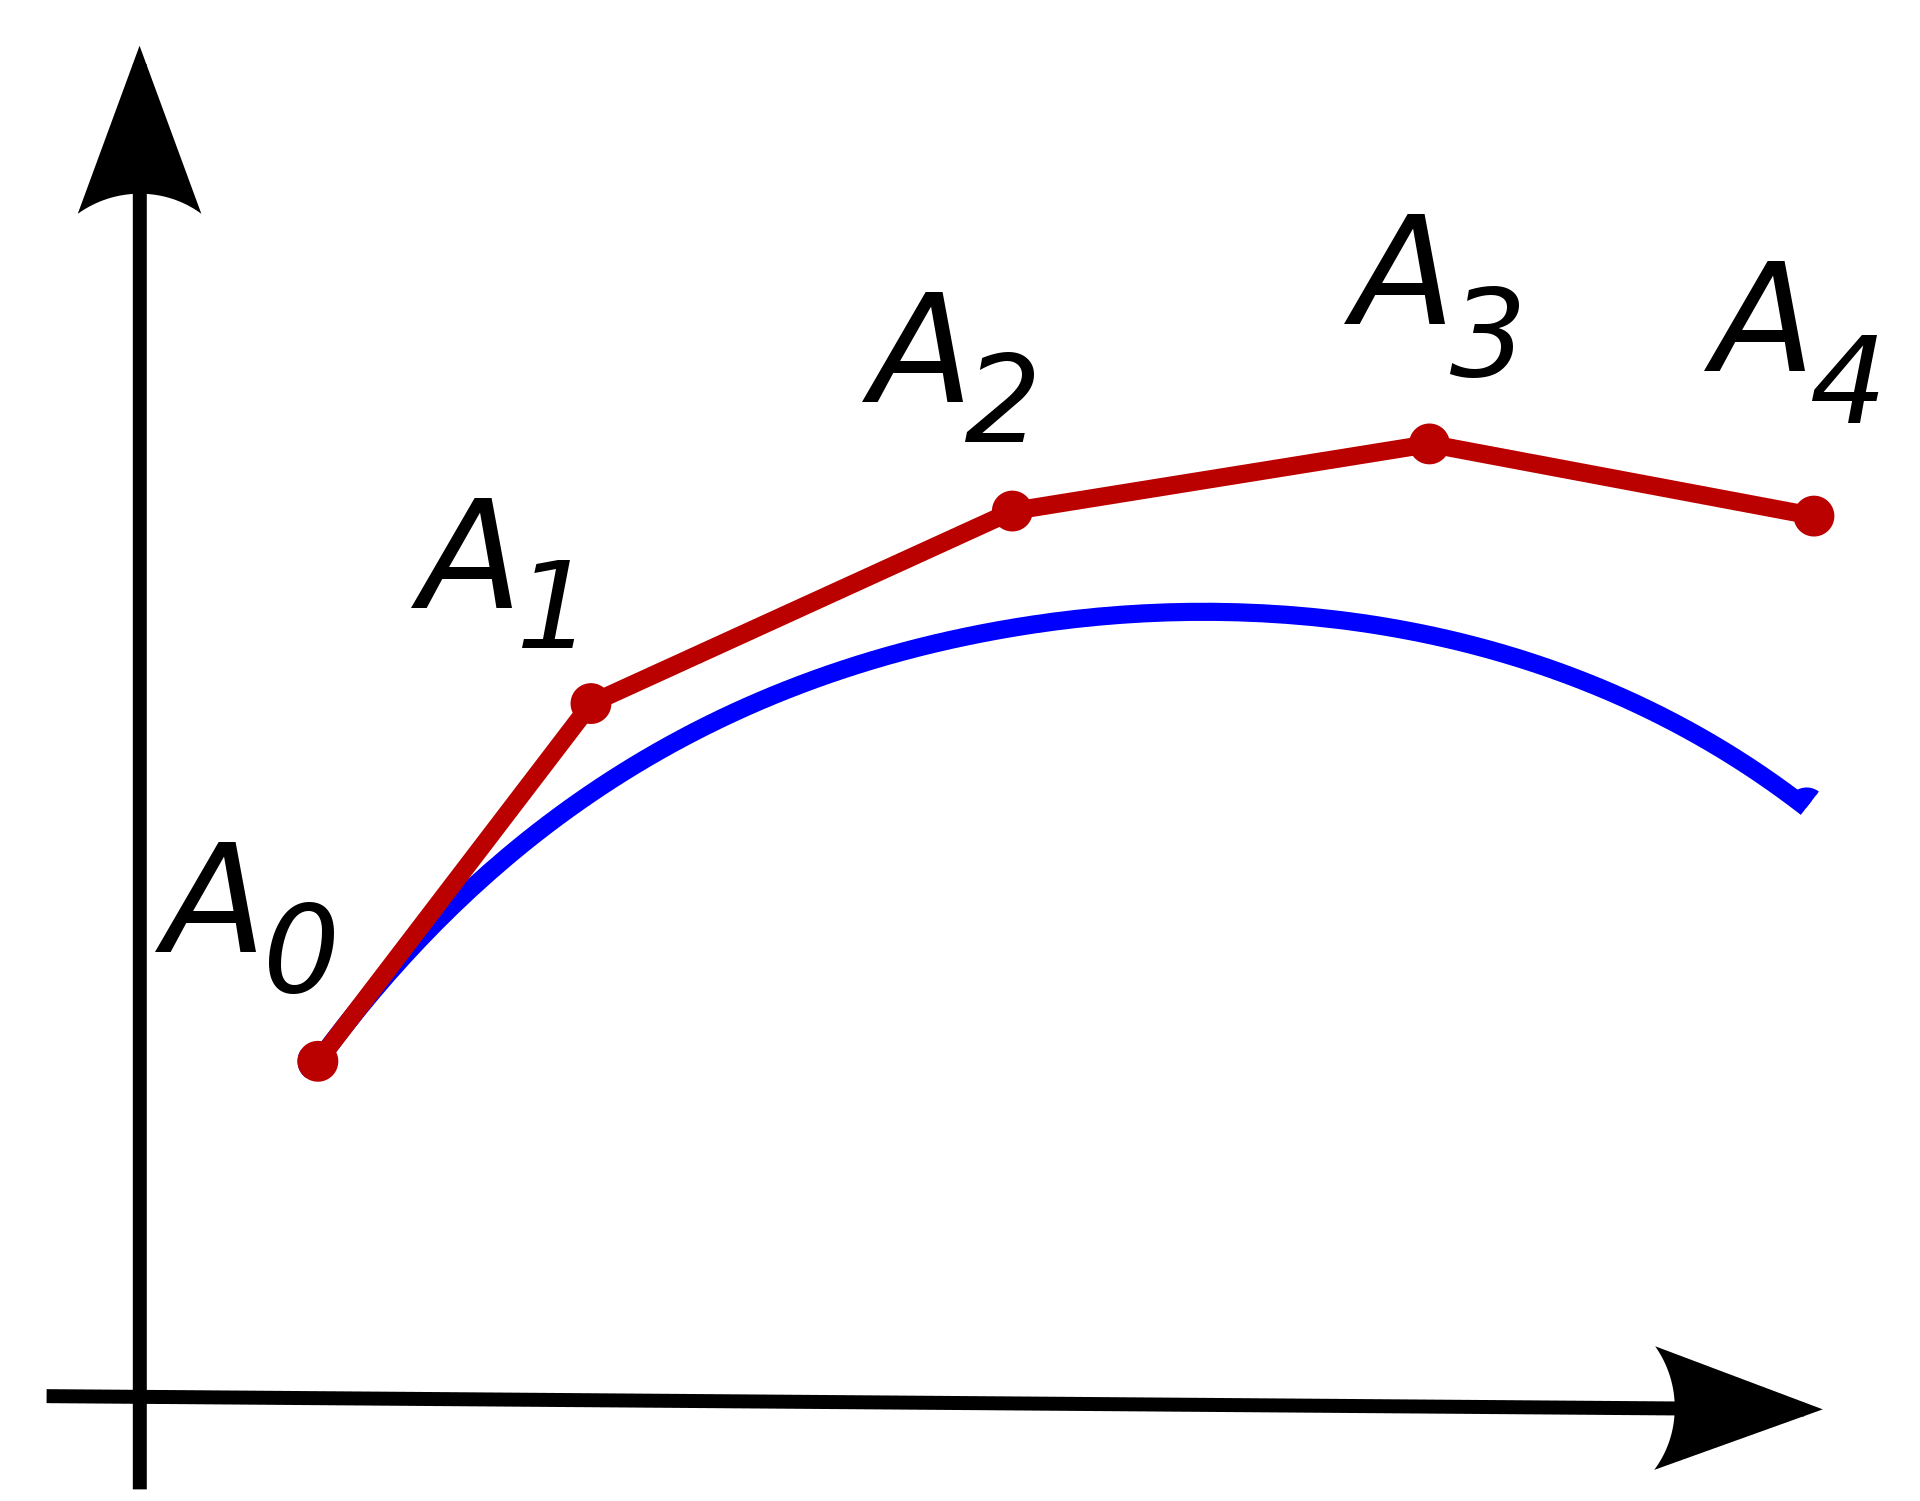
\includegraphics[scale=0.075]{expliciteuler.png}
	\caption{Illustration of the Euler method; the unknown curve is in blue, and its polygonal approximation is in red.}
\end{figure}

The error in the approximation of the solution by the explicit Euler method grows in proportion to the step size $h$; that is, $\|{\bf x}_N-{\bf x}(Nh)\|=\mathcal{O}(h)$. We therefore say that the method is first order accurate.

While the explicit Euler method is very easy to implement, it has a number of issues (you'll see one of them in the assignment). These include the fact that it becomes unstable (the error in its approximation starts to grow exponentially) when the step size is too large. The \emph{implicit Euler} (like the explicit Euler method, but the derivative is evaluated at the end of the time step i.e.$f(x_{n+1})$) method avoids this issue, but at the cost of needing to iteratively solve an implicit equation $x_{n+1}=x_n+hf(x_{n+1})$. It is still only first order.

Since $M\dot{\bf q} = {\bf p}$ and $M\ddot{\bf q} = \dot{\bf p}$ the equations of motion for the system from Newton's laws can be written as
\begin{equation}
	M\ddot{\bf q} = f({\bf q}) = -\nabla U({\bf q}).
	\label{eq:2vf}
\end{equation}
That is, we can turn the set of $2d$ first-order differential equations in ${\bf q}$ and ${\bf p}$ into $d$ second order differential equation in ${\bf q}$.
In much of what follows, I'm going to omit the mass matrix and write $\ddot{\bf q} = f({\bf q})$. The mass matrix is a symmetric matrix M that expresses the connection between the time derivative of the generalized coordinate vector q of a system and the kinetic energy T of that system, by the equation where denotes the transpose of the vector. This is purely for convenience. Everything still holds when $M$ takes other values for the masses --- just make sure to include a factor of $M^{-1}$ in the $f({\bf q})$ term.

A better approach to numerical integration is to use the Verlet (AKA St\"{o}rmer, AKA leap-frog) method. This is most easily understood in its \emph{two-step formulation} (i.e. the method requires information from two previously known time steps ($t_{n-1}$ and $t_n$) in order to compute the approximation at the future time step $t_{n+1}$). The approximation is given by 
\begin{equation}
	\frac{{\bf q}_{n+1} - 2{\bf q}_n + {\bf q}_{n-1}}{h^2} \simeq f({\bf q}_n) = \ddot{\bf q},
	\label{eq:2lf}
\end{equation}
where $f({\bf q})$ is the second order differential equation in equation \ref{eq:2vf}. It's not hard to see (see proof in reading [2]) that the LHS of \ref{eq:2lf} is an approximation of the second derivative at the point ${\bf q}_n$.

\begin{figure}[H]
	\centering
	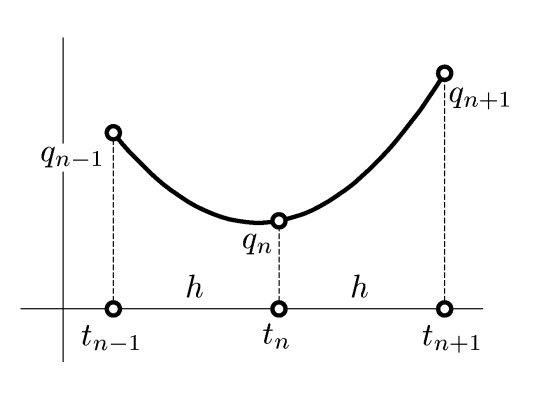
\includegraphics[scale=0.7]{twostep}
	\caption{Two-step formulation}
\end{figure}

The two-step formulation of the leapfrog method can therefore be seen as determining a parabola that interpolates the points ${\bf q}_{n-1},~{\bf q}_{n},$ and ${\bf q}_{n+1}$ and matches the second derivative at the midpoint.

It turns out that, for a number of reasons, it is better to work with the Verlet method in its one-step formulation. This can be derived by introducing the velocity ${\bf p}=\dot{\bf q}$ and turning equation \ref{eq:2vf} back into a first-order system of twice the dimension
It turns out that, for a number of reasons, it is better to work with the Verlet method in its one-step formulation. This can be derived by introducing the velocity $p=\dot{\bf q}$ and turning equation \ref{eq:2vf} back into a first-order system of twice the dimension
$$
	\dot{\bf q} = {\bf p},\qquad \dot{\bf p} = f({\bf q}).
$$

We then introduce discrete approximations of $q$ and $p$ as follows:
$$
p_n =\frac{q_{n+1}-q_{n-1}}{2h},\qquad p_{n-\frac12} = \frac{q_n-q_{n-1}}{h}, \qquad q_{n-\frac12} = \frac{q_n + q_{n-1}}{2},
$$
where some of the values have been calculated on a staggered grid. We can then use these to formulate a one-step version of the Verlet method. 
\begin{eqnarray*}
	{\bf p}_{n+\frac12} &=& {\bf p}_n+\frac{h}{2}f({\bf q}_n),\\
	{\bf q}_{n+1} &=& {\bf q}_n +h{\bf p}_{n+\frac12},\\
	{\bf p}_{n+1} &=& {\bf p}_{n+\frac12}+\frac{h}{2}f({\bf q}_{n+1}).
\end{eqnarray*}

\begin{figure}[H]
	\centering
	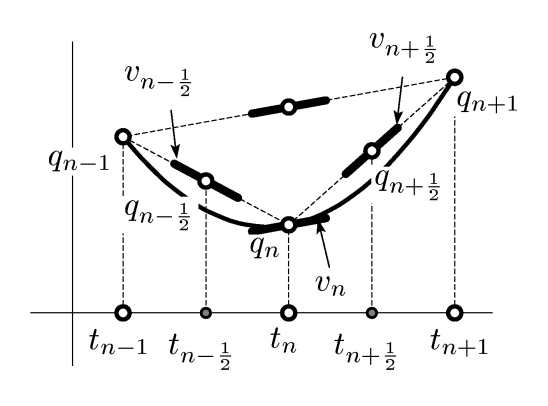
\includegraphics[scale=0.7]{onestep}
	\caption{One-step formulation}
\end{figure}

There is also a dual formulation of the method that gives the values of ${\bf q}$ and ${\bf p}$ on the staggered grid points $t_{n-\frac12},t_{n+\frac12},$ etc.
(It makes sense to think of the one-step method as a discrete map $\Phi_h$, similar to the flow map $\varphi_{f,t}$ that maps from the known solution, to its approximation one time step forward.)

If the velocity values are not needed at the end of each step, then the last line of one step can be combined with the first line of the next step to avoid one evaluation of $f$ per step by only calculating ${\bf p}$ on the staggered grid:
\begin{eqnarray*}
	{\bf p}_{n+\frac12} &=& {\bf p}_{n-\frac12}+hf({\bf q}_n),\\
	{\bf p}_{n+1} &=& {\bf q}_n +h{\bf p}_{n+\frac12}.
\end{eqnarray*}
This is the most computationally efficient form of the Verlet method. It is also numerically more stable than the two-step formulation.

It is not too hard to show (you should prove it for yourself) that the Verlet method is symplectic. That is, the discrete map that it defines preserves the symplectic form that we saw earlier. This is almost, but not quite the same as preserving the value of the associated Hamiltonian along solutions of the vector field. In fact, it is possible to show (but trickier than proving symplecticity) that the difference between the value of the Hamiltonian evaluated along the discrete approximation from the Verlet method differs only exponentially slowly from the exact value of the Hamiltonian for the true solution. This makes the Verlet method a popular choice for molecular dynamics. In addition to having good stability and being easy to implement, it is automatically almost energy-preserving.

The Verlet method is \emph{symmetric} (replacing $h$ with $-h$ and swapping the subscripts $n$ and $n+1$ gives the same method again) and \emph{reversible} (changing the sign on the velocity for the initial condition is the same as running the method in reverse). It is also second order accurate; that is the error in the solution $\|{\bf x}_{Nh}-{\bf x}(Nh)\|=\mathcal{O}(h^2)$.

Now that we have a suitable method for calculating the micro-state of a system at some point in the future, we can look for ways to measure macroscopic quantities from the solution. It is worth bearing in mind that for any simulations, the initial conditions used are unlikely to correspond to a representative configuration for the system. It is therefore good practise to let the simulation run for a period of time (perhaps a few thousand time steps) before attempting to measure any properties. This process is known as equilibration or thermalization.

Using simulated particle trajectories usually means we implicitly invoke an assumption of \emph{ergodicity}. This essentially says that averaging an observable along a solution, for a long enough time period for a system, is equivalent to averaging that observable over a large number of initial conditions for the same system, where the initial conditions correspond to the same macro-state of the system. While the hypothesis of ergodicity is useful, there are many real world cases where it doesn't hold --- for example any system that exhibits \emph{hysteresis} in which properties of the system are path dependent. Magnetic systems, in particular, tend to display such properties. For more discussion of this, see section 4.0 of \emph{Statistical Mechanics in a Nutshell}.

We have seen earlier that we identify the temperature of a thermodynamic system with the average square velocities of the particles in the system with some suitable normalisation. The temperature of our simulated system, with $N$ particles is therefore given by
$$
	T({\bf p}) = \frac{1}{Nk_B}\sum_{i=1}^N\frac{1}{2m_i}\|p_i\|^2.
$$

Another easily computable quantity is the virial function (we haven't mentioned this yet, but it is used to relate the total potential energy of a system to the total kinetic energy and can be used to calculate the pressure of a system --- see pp 255--256 of \emph{Statistical Mechanics in a Nutshell}):
$$
	C({\bf r}) = \sum_{i=2}^N\sum_{j=1}^{i-1}\nabla U(r_{ij})r_{ij},
$$
Both of these quantities give instantaneous values of the observables. Other quantities can be calculated as time averages of a solution of the system. For example, the constant volume specific heat:
$$
	C_v = k_B\left[\frac{2}{3N}-\frac{4}{9}\frac{\langle(T-\langle T\rangle)^2\rangle}{\langle T\rangle^2}\right]^{-1}
$$

where the angle brackets denote expected values over time.

\subsection{Recommended reading}
\begin{itemize}
	\item Sections 8.1 and 8.2 of \emph{Statistical Mechanics in a Nutshell}
	\item \emph{Geometric numerical integration illustrated by the St\"{o}rmer–Verlet method}, E. Hairer, Ch. Lubich, and G. Wanner, Acta Numerica (2003)
	\item Chapter 11 of \emph{Simulating Hamiltonian Dynamics}, B. Leimkuhler and S. Reich, Cambridge Univeristy Press (2004)
\end{itemize}

